\subsubsection{Deauthentication Denial of Service}
The deauthentication denial of service (DOS) [7] attack takes advantage of the unencrypted nature of the management frames by spoofing disassociation or deauthentication frames, depending on whether the attack wants to block a single device or all devices from the network. It is a denial of service that targets layer 2 in the OSI 7 Layer Model, there are other attacks designed for the other layers [4].

When a client wishes to gracefully disconnect from a 802.11 network it sends a disassociation frame [6] to the access point, likewise when an AP needs to disconnect from a client it sends a deauthentication [5] frame. If the AP needs to disconnect all clients, e.g. in the event of a reboot, it broadcasts the disassociation frame. 

The unencrypted and unauthorized nature of these frames leaves them open to MAC spoofing of either the client or AP, meaning an attacker can easily forge frames. It has been noted that deauthentication frames are preferable to spoof due to the access point and client having to perform the entire authentication cycle again in order to carry on using the network [1].
\clearpage
\begin{figure}[htbp!]
\centering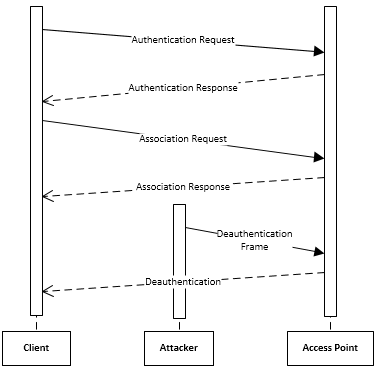
\includegraphics{research/attackvectors/figures/ddos.png}
\caption{Deauthentication DOS sequence.}
\end{figure}

The beauty of the deauthentication DOS is that it can be launched from relatively inexpensive hardware [3], with very little technical knowledge- especially when using a pre-existing application [2]. It should also be noted that this attack may not be started with malicious intent, as, for example, you have a network with a hidden SSID that users have discovered and hijacked, you can use this to deauthenticate all the users recover the network. On the more malicious side, this attack can be used to force users to connect to a spoofed access point after performing this attack, then chaining on a MITM attack.

\subsubsection*{Performing the Attack}
To demonstrate the simplicity of this attack I undertook it and documented the results. This is also partly to familiarise myself with the air-ng suite of tools which may be used during the implementation stage. 

\subsubsection*{Discovering the Access Point}
Although I knew the SSID and MAC address of the access point I would be targeting, I wanted to perform it from the perspective of somebody that didn’t. In order to achieve this I needed to use the airomon-ng tool that dumps a list of all access points that are broadcasting beacon frames, and stations broadcasting probe requests, along with their MAC address and SSID (where relevant).

\begin{figure}[h!]
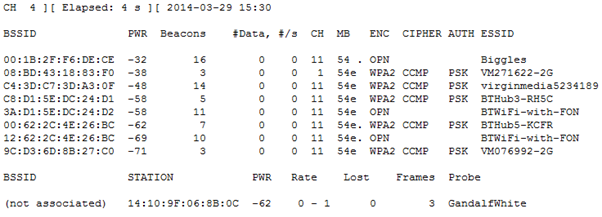
\includegraphics[width=\linewidth]{research/attackvectors/figures/ddos-1.png}
\caption{List of AP SSIDs in range of the wireless antenna.}
\end{figure}

\subsubsection*{Sending the Deauthentication Frame}
As the access point is transmitting on channel 11, I first needed to switch the monitor interface to channel 11, then I could use aireplay-ng [8] to send a deauthentication frame with spoofed MAC source and destination addresses.

\begin{figure}[h!]
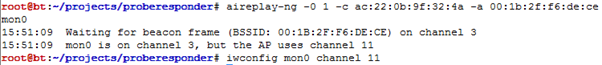
\includegraphics[width=\linewidth]{research/attackvectors/figures/ddos-2.png}
\caption{Changing the interface's channel.}
\end{figure}

\begin{figure}[h!]
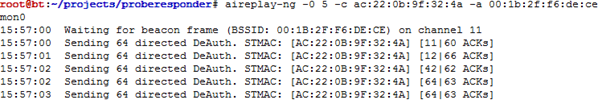
\includegraphics[width=\linewidth]{research/attackvectors/figures/ddos-3.png}
\caption{Sending the deauthentication frame.}
\end{figure}

\begin{figure}[h!]

\includegraphics[width=\linewidth]{research/attackvectors/figures/ddos-4.png}
\caption{Nexus 7 disassociating with the Netgear wireless router.}
\end{figure}

\subsubsection*{Including the Fake Access Point}
The image below demonstrates the attack paired with a simple fake access point. When the deauthentication frames were sent, the station reassociated with the fake access point I had created using another of the suite’s tools- airbase-ng.

\begin{figure}[h!]
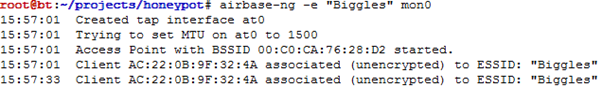
\includegraphics[width=\linewidth]{research/attackvectors/figures/ddos-5.png}
\caption{Station associating with the fake access point.}
\end{figure}